%!TEX root=./vissoft.tex

\newpage
\section {User Experience}
\label{sec:user}

  For service endpoints which run computations in real time, the maintainer of a system might want to understand the endpoint performance on a per-user basis, especially for situations where the system response time is a function of some individual user load\footnote{E.g. in GMail some users have two emails while other have twenty thousand and this induces different response times for different users}.

  To enable this, the \tool must be configured to associate an API call with a given user. The simplest way is to take advantage of the architecture of Flask applications in which a global \code{flask.request} object can be used to retrieve the session which can in turn lead to user identification: 

  %\begin{lstlisting}[float,caption=Simply define a custom app-specific function for user retrieval and pass it to the \tool to group information by user,style=custompython]
  \begin{lstlisting}[style=custompython]  
    # app specific way of extracting the user
    # from a flask request object    
    def get_user_id():
      sid = int(flask.request.args['session'])
      session = User.find_for_session(sid)
      return user_id

    # attaching the get_user_id function
    dashboard.config.get_group_by = get_user_id

  \end{lstlisting}

  % \niceseparator

  In Zeeguu, \epFeedItems retrieves a list of recommended articles for a given user. Cf. \Fref{fig:ep} it is the endpoint with the slowest response time and highest variability. The reason for this is that a user can be subscribed to anything from one to three dozen article sources and for each of the sources the system must compute the personalized difficulty of each article at every request. 

  % In the Zeeguu case study, one of the slowest endpoints, and one with the highest variability as shown in \Fref{fig:ep} is \epFeedItems: it retrieves a list of recommended articles for a given user. However, since a user can be subscribed to anything from one to three dozen article sources, and since the computation of the difficulty is personalized and it is slow, the variability in time among users is likely to be very large. 


  \begin{figure}[!ht]
    \centering
    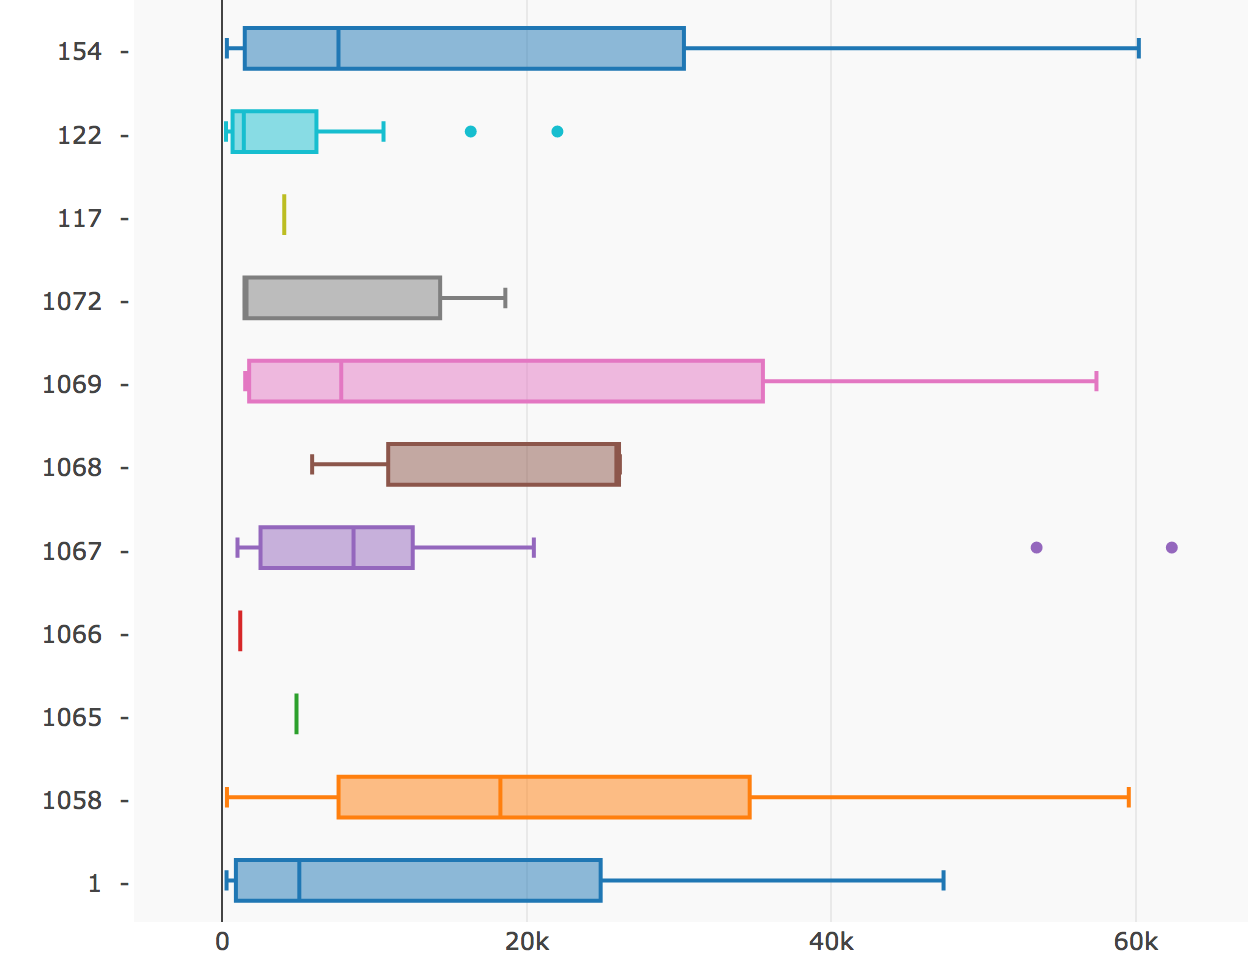
\includegraphics[width=0.85\linewidth]{time_per_user}
    \caption{The \epFeedItems shows a very high variability across users}
    \label{fig:tpu}
  \end{figure}

  A \perspective{Per-User Performance} perspective should show the different response times for different users. Figure \ref{fig:tpu} presents a subset of the corresponding view in the \tool. The figure shows that the response times for this endpoint can vary considerably for different users with some extreme cases where a user has to wait a full minute until their recommended articles are shown\footnote{After seeing this perspective, the maintainer refactored the architecture of the system to move part the difficulty computation out of the interactive loop}.

  
  % \niceseparator

  The limitation of the previous view is that it does not present the information also on a per version basis. To address this, a different visual perspective entitled \perspective{Multi-Version per-User Performance} can be defined. Figure \ref{fig:tuv} presents such a perspective by mapping the average execution time for a given user (lines) and given version (columns) on the area of the corresponding circle. The colors represent users. The figure shows performance varying  across users and versions with no clear trend: it is likely that the varying user workload is the reason for the variation in response times.

  \begin{figure}[!ht]
    \centering
    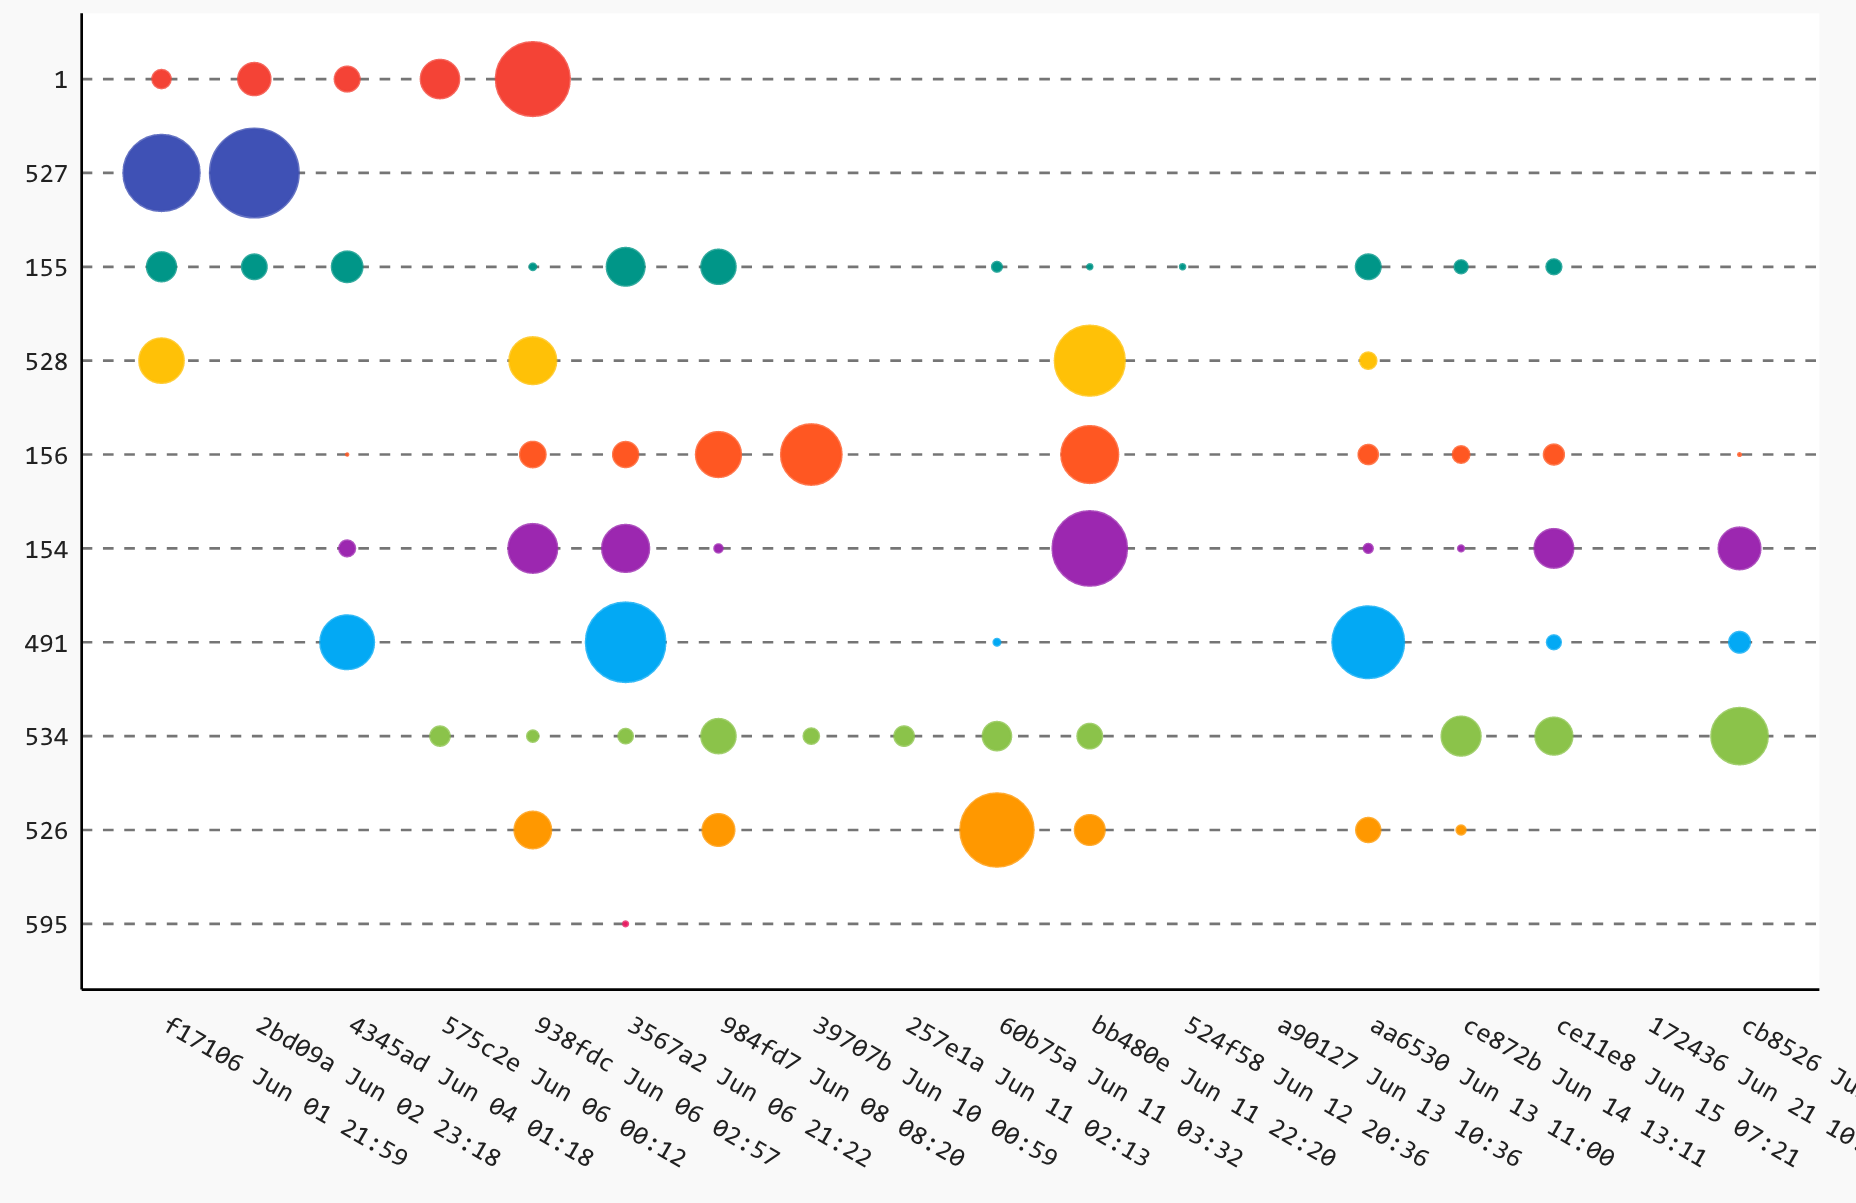
\includegraphics[width=0.9\linewidth]{time_per_user_per_version}
    \caption{This perspective shows that the evolution of response times for individual users (horizontal lines) across versions (the x-axis)}
    \label{fig:tuv}
  \end{figure}

  For the situations in which the user information is not available, the \tool also tracks out of the box information about different IPs. In some cases this might be a sufficiently good approximation of the user diversity and identity. 
  %
  In the interest of space limitations we are not showing this, and quite a few more visualizations provided by the \tool. The interested reader is referred to \Sref{sec:install} for further information on how to install the tool and how to get access to the data of the case study.
